\documentclass[11pt]{article}

\usepackage[margin=1in]{geometry}
\usepackage[T1]{fontenc}
\usepackage[utf8]{inputenc}
\usepackage{lmodern}
\usepackage{setspace}
\usepackage{hyperref}
\usepackage{graphicx}
\usepackage{booktabs}
\usepackage{enumitem}
\usepackage{tikz}
\usepackage{float}
\usetikzlibrary{arrows.meta,positioning,fit,shapes.multipart}

\setstretch{1.1}

\title{Heads-Up Texas Hold'em: Comparative Analysis of AI Agent Strategies}
\author{Sean Rowland \and Hayes Brown}
\date{}

\begin{document}
\maketitle

\noindent\textbf{Repository:}\url{https://github.com/Alvin-Furman-CS-Classroom/project-2-ai-system-all-in} \\
\textbf{Demo:} Local web demos at \texttt{web\_app} and \texttt{full\_game\_web\_app}

\begin{abstract}
This project implements a comparative AI system for heads-up Texas Hold'em poker, centered on pre-flop strategy while supporting full-hand execution in integrated web interfaces. The core goal is to evaluate how different AI paradigms---symbolic reasoning, informed search, Monte Carlo simulation, LLM-based decision support, and reinforcement learning---perform under a shared game framework. We implemented five modules: a propositional-logic playability filter (Module 1), an EV-driven A*/brute-force bet sizing component (Module 2), a Monte Carlo action evaluator (Module 3), an Ollama-first LLM strategy layer with structured legal-action selection (Module 4), and a tabular RL policy with checkpointed training/evaluation (Module 5). Agent-versus-agent benchmarking indicates clear behavioral differences: search and Monte Carlo agents are strong against random and RL checkpoints in current settings, while LLM behavior is limited by high decision latency and local runtime constraints. The system demonstrates both practical playability and educational value by exposing trade-offs between interpretability and empirical performance across AI paradigms in one coherent architecture.
\end{abstract}

\section{Introduction}
Poker is a useful AI benchmark because it combines uncertainty, strategic adaptation, and optimization. Our final project focus is full-game comparison in heads-up Texas Hold'em, where agents must make decisions across preflop, flop, turn, and river. The system supports two usage modes: human-vs-agent web play and agent-vs-agent benchmarking for comparative analysis.

The implemented system contains five topic-aligned modules. Module 1 encodes playability rules via propositional logic and CNF-style knowledge-base reasoning. Module 2 uses informed search and EV models to recommend fold/call/raise sizing. Module 3 estimates action value through Monte Carlo simulation. Module 4 integrates an LLM agent with legal-action constraints and reasoning logging. Module 5 trains a tabular RL policy over bucketed state/action spaces in a full-game engine environment.

Implementation and evaluation tooling uses standard Python libraries for web delivery, configuration management, and numerical analysis, including Flask [1], python-dotenv [2], NumPy [3], and Matplotlib [4]. The local LLM runtime uses Ollama [5], which keeps inference reproducible without external hosted APIs.

The project does not claim game-theoretic optimality or full-scale equilibrium solving. Instead, it provides a practical and testable multi-agent environment that demonstrates how diverse AI paradigms behave under a common interface and shared game-state transitions.

\section{System Architecture}
The architecture separates policy logic from game execution. Two engines support gameplay: a preflop-focused engine (\texttt{game\_engine}) and a full-hand engine (\texttt{full\_game\_engine}). Web applications (\texttt{web\_app}, \texttt{full\_game\_web\_app}) manage session state, routing, and UI interactions. Agent adapters translate engine state into module-specific inputs and map module recommendations back to legal engine actions.

Utilities are shared to reduce integration duplication: \texttt{project\_paths.py} standardizes import bootstrap, \texttt{engine\_adapter\_utils.py} centralizes legal-action mapping helpers, and \texttt{engine\_mc\_adapter\_utils.py} centralizes Monte Carlo adapter flow shared by pre-flop and full-game stacks.

The high-level data flow is: current \texttt{HandState} $\rightarrow$ agent policy call $\rightarrow$ legal-action mapping/validation $\rightarrow$ engine \texttt{apply\_action} $\rightarrow$ updated state and metrics logging. Evaluation scripts consume this same path, which improves fidelity between play and benchmark behavior.

\begin{figure}[h]
  \centering
  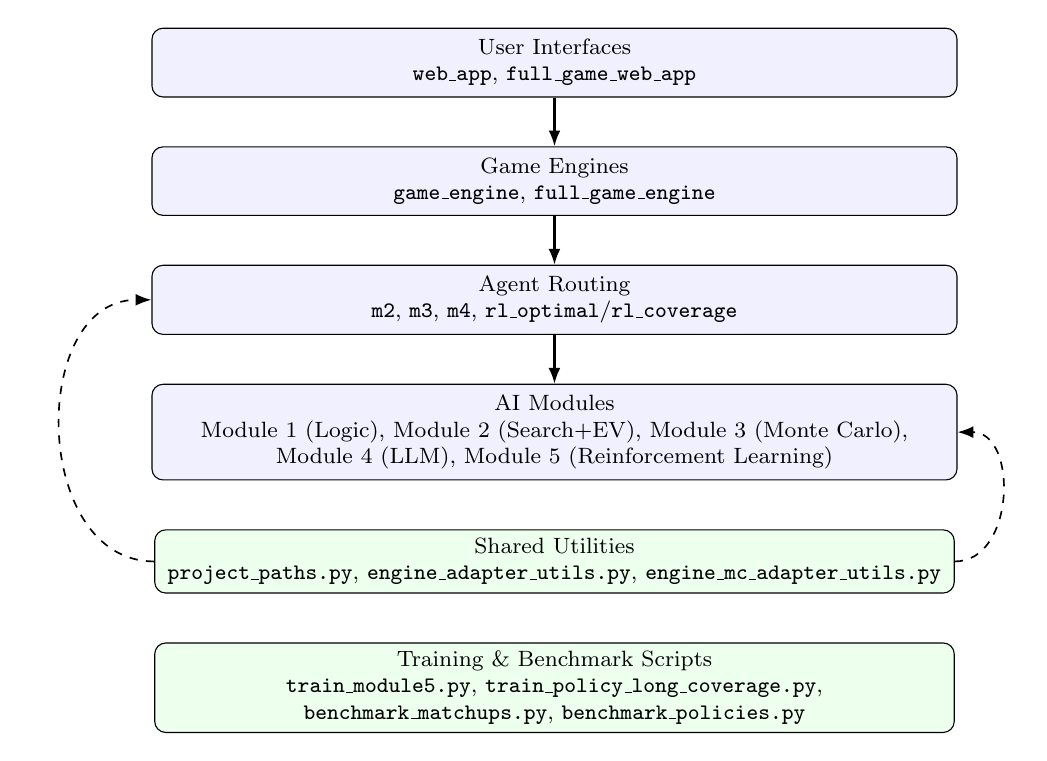
\begin{tikzpicture}[
    font=\footnotesize,
    node distance=0.62cm and 0.9cm,
    box/.style={draw, rounded corners, align=center, minimum height=8mm, fill=blue!6, inner sep=4pt, text width=0.82\linewidth},
    slim/.style={draw, rounded corners, align=center, minimum height=7mm, fill=green!7, inner sep=3pt, text width=0.82\linewidth},
    flow/.style={-{Latex[length=2mm]}, thick},
    aux/.style={-{Latex[length=2mm]}, dashed, semithick}
  ]

  % Vertical flow
  \node[box] (ui) {User Interfaces\\\texttt{web\_app}, \texttt{full\_game\_web\_app}};
  \node[box, below=of ui] (eng) {Game Engines\\\texttt{game\_engine}, \texttt{full\_game\_engine}};
  \node[box, below=of eng] (adapt) {Agent Routing\\\texttt{m2}, \texttt{m3}, \texttt{m4}, \texttt{rl\_optimal}/\texttt{rl\_coverage}};
  \node[box, below=of adapt] (mods) {AI Modules\\
  Module 1 (Logic), Module 2 (Search+EV), Module 3 (Monte Carlo),\\
  Module 4 (LLM), Module 5 (Reinforcement Learning)};
  \node[slim, below=of mods] (utils) {Shared Utilities\\
  \texttt{project\_paths.py}, \texttt{engine\_adapter\_utils.py}, \texttt{engine\_mc\_adapter\_utils.py}};
  \node[slim, below=of utils] (train) {Training \& Benchmark Scripts\\
  \texttt{train\_module5.py}, \texttt{train\_policy\_long\_coverage.py},\\
  \texttt{benchmark\_matchups.py}, \texttt{benchmark\_policies.py}};

  % Main flows
  \draw[flow] (ui) -- (eng);
  \draw[flow] (eng) -- (adapt);
  \draw[flow] (adapt) -- (mods);

  % Utility support
  \draw[aux] (utils.west) to[out=180,in=180,looseness=1.2] (adapt.west);
  \draw[aux] (utils.east) to[out=0,in=0,looseness=1.2] (mods.east);

  \end{tikzpicture}
  \caption{System architecture and module integration pipeline.}
  \label{fig:architecture}
\end{figure}

Figure~\ref{fig:architecture} shows the vertical integration path used by both gameplay and benchmarking: UI request handling, engine progression, agent routing, module inference, and shared utility support. This alignment improves validity because benchmarked and interactive decisions pass through the same legal-action normalization and error-handling boundaries.

\section{Module Implementation Summary}

\subsection{Module 1: Rule-Based Decision Framework}
Module 1 determines whether a hand is playable given position, stack depth, and opponent tendency. Its inputs are hand and context features, and its outputs are a playability decision, a reason string, and derived knowledge-base facts. The implementation uses CNF-style rule encoding with backward-chaining style derivation to preserve explainability. In integration, Module 1 is used as a pre-filter for Module 2 search-based action selection.

\subsection{Module 2: Optimal Bet Sizing Search}
Module 2 selects EV-maximizing actions and raise sizes using A* or brute-force search over a discretized action space. It consumes hand context plus an optional Module 1 result and returns \texttt{action}, \texttt{bet\_size}, \texttt{expected\_value}, and a human-readable reason. A key design choice is tendency-conditioned EV modeling: fold/call/raise response probabilities are adjusted by opponent profile so that the same candidate bet can have different expected value against tight, loose, aggressive, or passive behavior.

Module 1 feeds directly into this pipeline through optional playability filtering. When Module 1 marks a hand as not playable in the current context, Module 2 can short-circuit the search and return a fold decision instead of exploring raise/call branches, which keeps symbolic constraints and search optimization aligned.

\subsection{Module 3: Monte Carlo Optimal Opening Actions}
Module 3 estimates action value through simulation rather than closed-form EV expressions. It takes position, stack sizes, opponent tendency, and hand/action parameters, and returns value estimates with uncertainty statistics (standard deviation and confidence intervals). The implementation uses configurable trial budgets and conditioned-range logic for fuller-hand approximations.

Configurable trial budgets allow the system to trade accuracy for runtime depending on where it is used (for example, faster web decisions versus deeper offline benchmarking). Conditioned-range logic means opponent hand sampling is adjusted by context (such as board texture and action type) rather than always sampling from a uniform or purely preflop distribution, which makes postflop approximations more realistic.

\subsection{Module 4: LLM-Based Strategy Agent}
Module 4 uses an LLM to choose a legal action index from a structured game-state snapshot. Inputs include the serialized context and legal action list, while outputs include the selected legal action and metadata such as reason text, model/provider, and repair/fallback indicators. The design is Ollama-first for local reproducibility and includes robust parsing plus strict legal-action normalization. Runtime integration relies on local Ollama serving behavior and model invocation APIs [5].

\subsection{Module 5: Reinforcement Learning}
Module 5 learns a policy from interaction outcomes using tabular Q-learning and Monte Carlo-style return updates. It consumes encoded state tuples, discrete action buckets, and reward signals, and produces checkpointed Q-table policies with evaluation metrics. Design choices include bucketed state abstractions, masked legal-bucket action selection, and rich checkpoint metadata for reproducibility and resume support.

\section{Evaluation Methodology}
We used full-game benchmark scripts to run pairwise matchups across \texttt{m2}, \texttt{m3}, \texttt{m4}, \texttt{rl\_optimal}, \texttt{rl\_coverage}, and \texttt{random}. Metrics in the matchup reports include bb/100 and 95\% confidence intervals, hand win rate and tie rate, action legality rate, decision error and fallback-to-random rates, and average decision latency in milliseconds.

For reproducibility, benchmark generation followed a fixed command path using the project entry points (\texttt{python3 -m full\_game\_engine.benchmark\_matchups} for full-game evaluation and Module 5 scripts for RL policy checkpoints). We used deterministic seeds where supported (seed 1337 in the current report configuration), fixed blind levels, and fixed starting stacks to reduce setup-driven variance. Reports were produced from script outputs and copied directly into markdown artifacts so paper metrics map to recorded run logs rather than hand-entered values.

One concrete reproduction example that generates the cited report artifact is:
\texttt{python3 -m full\_game\_engine.benchmark\_matchups --hands 10000 --llm-hands 10 --seed 1337 --include-self-matchups --report-path docs/AGENT\_MATCHUP\_REPORT.md}.

The evaluation design intentionally separates throughput-sensitive and latency-sensitive regimes. Non-LLM pairings use high hand counts to estimate bb/100 with lower variance, while LLM-including pairings use smaller hand counts because of inference cost. This reflects practical deployment constraints but introduces different confidence levels across matchup classes, which we account for in the Results interpretation.

\begin{table}[h]
  \centering
  \caption{Selected benchmark outcomes from \texttt{AGENT\_MATCHUP\_REPORT.md}.}
  \label{tab:matchup-results}
  \begin{tabular}{lccc}
    \toprule
    Matchup & bb/100 & Win Rate & Error Rate \\
    \midrule
    m2 vs random (m2 row) & 245.510 & 41.57\% & 0.00\% \\
    m3 vs random (m3 row) & 637.625 & 83.03\% & 0.00\% \\
    m2 vs m3 (m2 row) & 118.065 & 28.65\% & 0.00\% \\
    \bottomrule
  \end{tabular}
\end{table}

The current \texttt{AGENT\_MATCHUP\_REPORT.md} setup uses 10{,}000 hands for non-LLM pairings and 10 hands for pairings involving the LLM agent, with seed 1337, equal 100BB starting stacks, and blinds SB=10/BB=20.

Table~\ref{tab:matchup-results} summarizes representative outcomes from the current benchmark report and provides a compact cross-check against the discussion in the Results section.

\section{Results}
Results indicate strong performance from search and Monte Carlo agents against random and current RL checkpoints under the evaluated settings, with the search heuristic agent showing stronger overall outcomes in the latest long-run benchmark configuration. Representative outcomes from \texttt{AGENT\_MATCHUP\_REPORT.md}:

\begin{figure}[H]
  \centering
  \includegraphics[width=0.85\linewidth]{results.png}
  \caption{Comparative performance visualization across agent matchups (heatmap/table view).}
  \label{fig:results-plot}
\end{figure}

Figure~\ref{fig:results-plot} shows cross-agent performance using big blinds per 100 hands. The Logic and Monte Carlo agents perform strongly against most opponents. The reinforcement agents only slightly outperform random play, although they retain a clear advantage over the LLM agent in this configuration.

These statements are directly reflected in Table~\ref{tab:matchup-results}: \texttt{m3} vs \texttt{random} reports 637.625 bb/100 and 83.03\% win rate (row \texttt{m3 vs random}), while \texttt{m2} vs \texttt{random} reports 245.510 bb/100 (row \texttt{m2 vs random}). Table~\ref{tab:matchup-results} also shows a positive 118.065 bb/100 for \texttt{m2} in \texttt{m2 vs m3} (row \texttt{m2 vs m3}), which provides a concrete head-to-head signal under the same evaluation pipeline.

The LLM agent (\texttt{m4}) remained legally compliant with zero measured fallback/error rates in this run. However, average decision latency remained high (8--11 seconds), which constrained practical strength despite successful integration.

Across all rows, legality remained 100\%, suggesting adapter validation and action mapping are robust. This supports the architecture goal of enforcing legal-action boundaries regardless of policy internals.

Confidence-interval interpretation is central for honest comparison. In high-sample non-LLM matchups, intervals are narrow enough that sign and rough magnitude comparisons remain stable at the level reported in Table~\ref{tab:matchup-results}. In contrast, LLM-including matchups with very small sample sizes show much higher variance, so point estimates should be treated as directional indicators rather than final ranking evidence. We therefore use LLM results primarily to assess integration correctness, legal-action reliability, and latency characteristics, not definitive skill ordering.

A sensitivity pattern also appears when contrasting matchup volumes: as hand counts increase, short-run variance has less influence on aggregate bb/100, and strategy-level differences in opening policy and postflop continuation become clearer. This is one reason larger non-LLM runs are more useful for comparing \texttt{m2}, \texttt{m3}, and RL checkpoints. Future evaluation should add repeated seeded batches and aggregated confidence envelopes so comparisons rely on multiple independent runs rather than single-seed summaries.

Threats to validity remain. First, unequal sample sizes between LLM and non-LLM pairings reduce comparability across the matrix. Second, all results are generated under one blind structure and one stack-depth regime, so external validity to other cash-game settings is limited. Third, current RL checkpoints reflect specific abstraction and training distributions; stronger or differently trained policies could change relative rankings. These caveats are why we frame conclusions as evidence-backed but conditional on the tested setup.

From a practical systems perspective, these results show a deployment trade-off that matters beyond bb/100. Search- and simulation-based agents deliver consistent low-latency decisions, making them easier to use in interactive settings without user-visible delays. The LLM agent, while expressive and often strategically sensible in local contexts, introduces variable response times that can degrade gameplay flow even when decisions are legal. This motivates a hybrid architecture for future versions: use a fast baseline policy for immediate action proposals and reserve LLM calls for selective high-uncertainty states or post-hand analysis. One practical gating signal is disagreement between the fast agents (for example, when \texttt{m2} and \texttt{m3} select different action types), triggering an LLM call only for those cases.

\section{Proposal Delta}
Compared to the initial proposal, the final system retained the original five-module structure but evolved in scope and emphasis. The largest change was expanding from a primarily preflop plan to full-game play, because the core approaches transferred well across streets and full-game evaluation is both more realistic and more informative for behavioral comparison. We also shifted from a single combined agent design to four independent agents, each representing a distinct AI strategy. Although integration was feasible, each module produced coherent play independently, and separation enabled clearer head-to-head evaluation of strengths and weaknesses. In addition, Module 3 was revised from an advanced-search concept to a Monte Carlo simulation approach, which proved more practical for estimating decision quality under uncertainty in full-game states. Finally, Module 4 moved from a GTO chart-based plan to an LLM-based approach: generating high-quality GTO charts ourselves was computationally expensive, while comprehensive existing charts were largely inaccessible behind paywalls. No module was removed; instead, implementation broadened and was rebalanced toward full-game integration and comparative empirical analysis.

\section{Limitations and Failure Analysis}
\textbf{LLM latency under local inference.} In current report matchups, \texttt{m4} remains legally reliable but still exhibits materially higher decision latency than other agents. Likely causes include local model inference cost and prompt/parse overhead. Future work includes asynchronous decisioning, smaller/faster local models, and tighter prompt/output schema to reduce repair passes while preserving legality.

\textbf{RL policy strength variance vs benchmark opponents.} Current RL checkpoints underperform search/Monte Carlo in several evaluated pairings despite long training schedules. Likely causes include tabular state abstraction limits, self-play distribution mismatch, and reward-credit granularity. Improvements such as richer feature encoding, policy/value function approximation, and targeted opponent pools would likely increase robustness across opponent classes.

\textbf{Simplified opponent modeling in analytic modules.} Module 2 tendency-conditioned EV and Module 3 range-conditioning are practical approximations, but they still compress real strategic diversity into tractable model assumptions. In edge cases, this can over- or under-estimate continuation frequencies relative to real opponents. A high-value improvement is to calibrate these models against larger simulated populations and empirical play traces.


\section{Individual Contributions}
Sean Rowland and Hayes Brown contributed approximately equally to the project, with an estimated relative effort distribution of 50\% and 50\%, respectively.
Both members collaborated on the design, implementation, and iterative refinement of Modules 1-3, including integration and testing activities.
For the remaining components, Sean Rowland held primary responsibility for Module 4, while Hayes Brown held primary responsibility for Module 5.
In addition, both members jointly developed the presentation slides and co-authored the final paper.

\section{Conclusions and Future Work}
This project delivered a complete multi-agent AI poker system with strong modularity, integration readiness, and test reliability, culminating in full-game comparative evaluation. Across modules, we demonstrated symbolic reasoning, informed search, simulation-based optimization, LLM-mediated legal-action selection, and RL-based policy learning within a unified engine framework.

The strongest empirical performers in current benchmarks were search and Monte Carlo variants under the tested settings, while LLM and RL paths highlighted practical trade-offs in latency and training distribution alignment.

Future work should prioritize stronger RL representations and opponent curricula, lower-latency/high-reliability LLM decision pipelines, and broader benchmark suites with longer LLM-inclusive runs and richer statistical analysis. These steps would improve both performance realism and scientific validity of cross-paradigm comparisons.

\section{References}
\begin{enumerate}[leftmargin=*]
  \item Flask Documentation, ``Flask,'' Pallets. [Online]. Available: \url{https://flask.palletsprojects.com/}. [Accessed: Apr. 26, 2026].
  \item B. A. Saurabh Kumar, ``python-dotenv,'' PyPI. [Online]. Available: \url{https://pypi.org/project/python-dotenv/}. [Accessed: Apr. 26, 2026].
  \item NumPy Developers, ``NumPy,'' NumPy.org. [Online]. Available: \url{https://numpy.org/}. [Accessed: Apr. 26, 2026].
  \item Matplotlib Development Team, ``Matplotlib: Visualization with Python,'' Matplotlib.org. [Online]. Available: \url{https://matplotlib.org/}. [Accessed: Apr. 26, 2026].
  \item Ollama, ``Ollama,'' Ollama Inc. [Online]. Available: \url{https://ollama.com/}. [Accessed: Apr. 26, 2026].
\end{enumerate}

\end{document}